\chapter{Aktueller Forschungsstand und Forschungsfrage}
\label{ch_04Aktueller Forschungsstand und Forschungsfrage}

\begin{figure}[h]
	\centering
	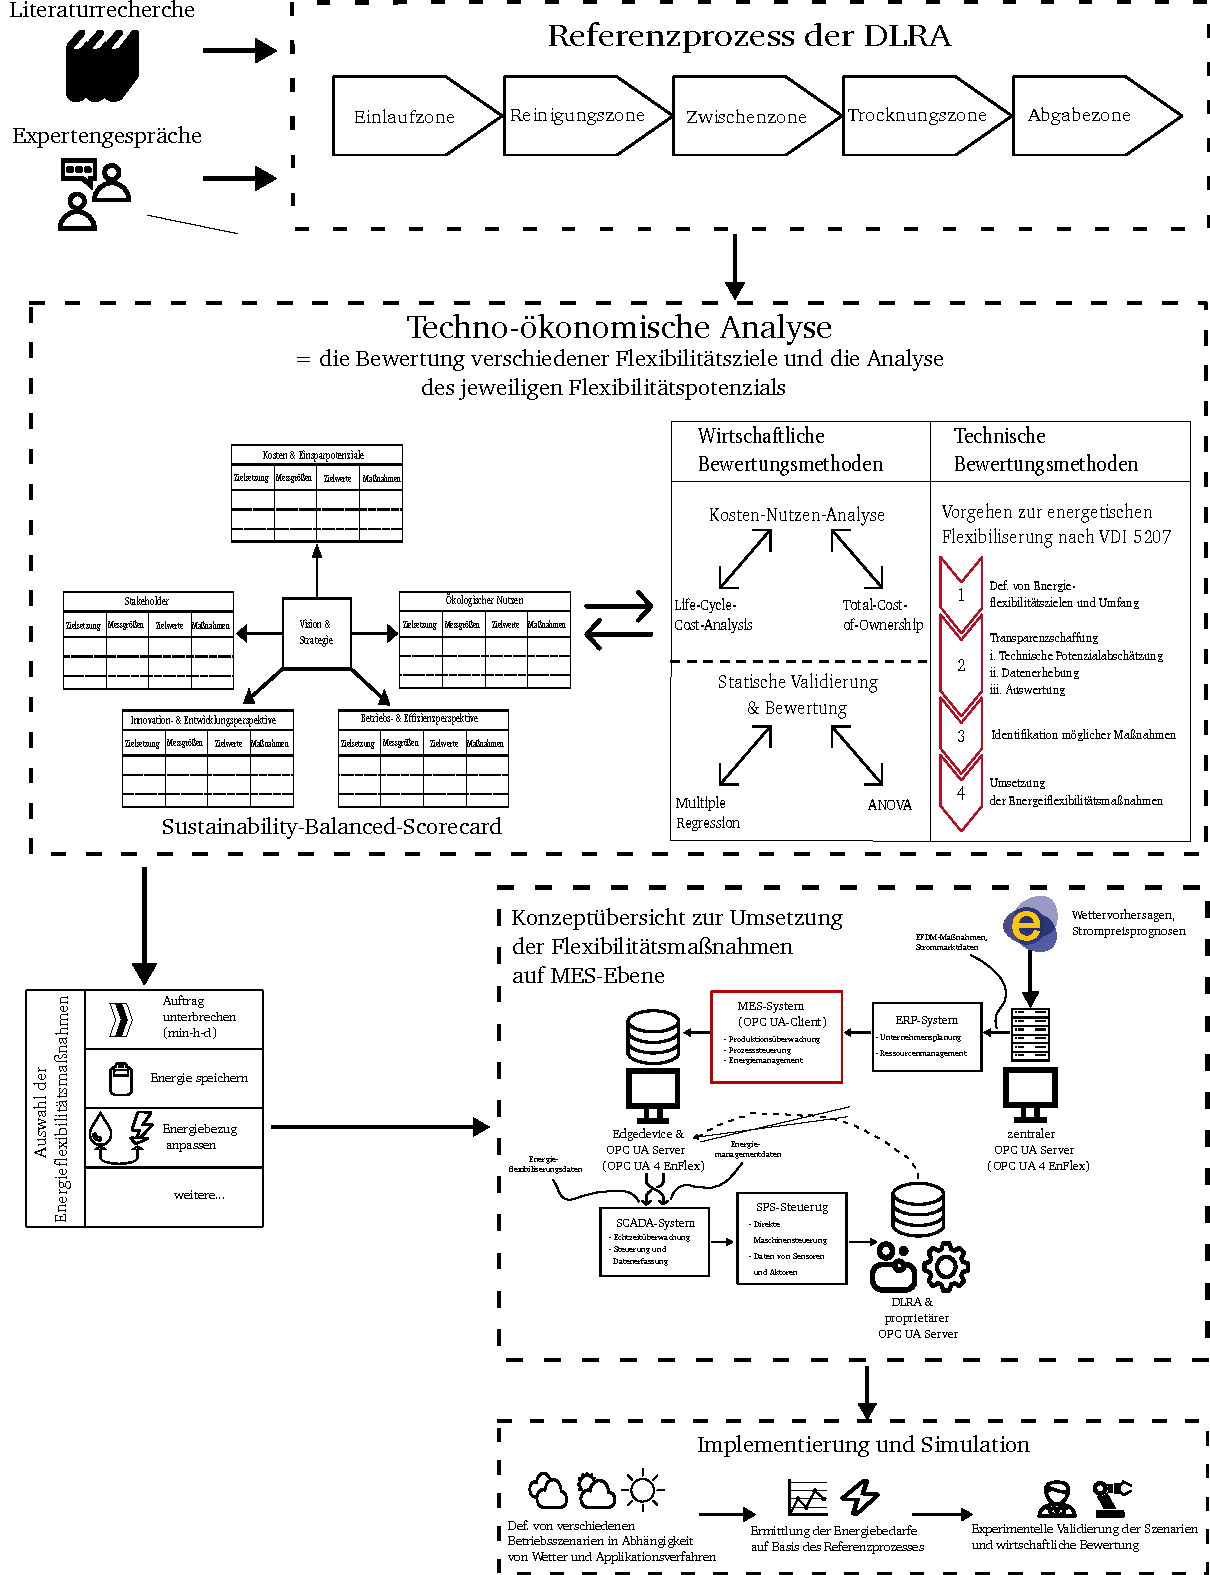
\includegraphics[width=\textwidth]{C:/Users/Anwender/Desktop/LaTeX_Template_Abschlussarbeit_TexStudio/figures/04_Aktueller Forschungsstand und Forschungsfrage/BigPicture.pdf}
	\caption{Beschreibung des Bildes}
	\label{fig_BigPicture}
\end{figure}


\section{Durchlaufreinigungsanlage (DLRA)}
\label{ch_04Durchlaufreinigungsanlage (DLRA)}
Weiteres bla bla bla...

\subsection{Beschreibung des praktischen Anwendungsfalls}
\label{ch_04Beschreibung des praktischen Anwendungsfalls}
Text

\subsection{Bedeutung für die Energieflexibilisierung}
\label{ch_04Bedeutung für die Energieflexibilisierung}
Text
\section{ETA-Fabrik}
\label{ch_04ETA-Fabrik}

\begin{itemize}
	\item Überblick über die ETA-Fabrik und deren Relevanz für die Studie
\end{itemize}
\section{SynErgie-Projekt}
\label{ch_04SynErgie-Projekt}
\begin{itemize}
	\item Beschreibung des Projektes und dessen Beitrag zur Energieflexibilisierung
\end{itemize}
\section{Ansteuerung von Datenpunkten mittels OPC-UA-Schnittstelle}
\label{ch_04Ansteuerung von Datenpunkten mittels OPC-UA-Schnittstelle}
\begin{itemize}
	\item Technische Details und Implementierung
\end{itemize}
\input{texts/04_Aktueller Forschungsstand und Forschungsfrage/Implementierung von Energieflexibilitätsmaßnahmen auf Fertigungsebene.tex}
\section{Forschungsziel und Fragen}
\label{ch_04Forschungsziel und Fragen}

Das Ziel der Masterthesis besteht darin, ein Konzept zur Implementierung geeigneter Flexibilitätsmaßnahmen auf der MES-Ebene für die DLRA zu entwickeln und anhand verschiedener Betriebsszenarien den zugehörigen Energiebedarf auf Basis des Referenzprozesses zu ermitteln. Nach der experimentellen Validierung der Szenarien soll eine wirtschaftliche Bewertung der implementierten Maßnahmen erfolgen.

Im Rahmen dieser Arbeit sollen folgende Forschungsfragen untersucht werden:

\begin{enumerate}[label=\textbf{\arabic*.}]
	\item \textbf{Kosteneffizienz der Energieflexibilitätsmaßnahmen:}\\ \emph{In welchem Umfang übersteigen die Einsparungen durch die Implementierung von Energieflexibilitätsmaßnahmen die damit verbundenen Kosten, und welche spezifischen Kostenfaktoren beeinflussen diese Bilanz?}
	
	Es ist entscheidend, zwischen den fixen Kosten, die durch die Implementierung der Maßnahmen entstehen, und der fortlaufenden Reduktion der variablen Betriebskosten der entsprechenden Anlage zu differenzieren. Diese Unterscheidung ermöglicht eine präzisere Bewertung der Kosteneffizienz. Ein zentrales Element ist die Berechnung der Amortisationszeit der Investition, um den Zeitraum zu bestimmen, in dem die Maßnahme wirtschaftlich wird. Darüber hinaus muss die Skalierbarkeit der Lösung über die OPC UA Schnittstelle berücksichtigt werden, da dies die Übertragung der Vorteile auf andere Anlagen erleichtert und somit eine breitere Anwendung ermöglicht.
	
	Ein weiterer wichtiger Aspekt im Zusammenhang mit dieser Forschungsfrage ist die Übertragbarkeit der in dieser Arbeit entwickelten und getesteten Flexibilitätsmaßnahmen auf industrielle Anwendungen. Es müssen spezifische Anpassungen ermittelt werden, um die Maßnahmen in einem realen industriellen Umfeld erfolgreich umzusetzen. Dies umfasst die Berücksichtigung der technischen Anforderungen sowie die Anpassung an unterschiedliche Betriebsbedingungen und Produktionsprozesse. Eine erfolgreiche Übertragung der Maßnahmen kann die wirtschaftlichen Vorteile maximieren und zu einer breiteren Akzeptanz und Anwendung in der Industrie führen.
	
	\item \textbf{Einflussfaktoren auf den Energiebedarf:}\\\emph{Welche spezifischen Einflussfaktoren aus Wetterdaten und Lastprofilen beeinflussen in welchem Ausmaß den Energiebedarf unter verschiedenen Betriebsszenarien und -strategien der Durchlaufreinigungsanlage (DLRA), und wie wirkt sich die Volatilität des Wetters in Kombination mit unterschiedlichen Lastprofilen auf die Umsetzung der Energieflexibilitätsmaßnahmen} aus?
	
	In Kapitel \ref{ch_05Ausarbeitung eines geeigneten Referenzprozesses} wird neben der Ausarbeitung eines geeigneten Referenzprozesses, auch verschiedene Marktszenarien definiert. Aus der Kombination dieser Marktszenarien und des Referenzprozesses werden die Betriebsszenarien hergeleitet, die für die Analyse und Beantwortung der Forschungsfrage verwendet werden. 
	
\end{enumerate}

Durch die Beantwortung dieser Fragen wird ein umfassendes Verständnis darüber gewonnen, wie eine energetische Flexibilisierung des Betriebs einer DLRA unter Berücksichtigung technischer und ökonomischer Faktoren optimiert werden kann.\\

Auf Grundlage der Forschungsfragen und spezifischer Aspekte der Untersuchung werden weitere Untersuchungshypothesen aufgestellt. Einige der Hypothesen sind auf Prädiktoren zurückzuführen, welche im Rahmen der multiplen Regression und einer ANOVA untersucht werden.\\

\textbf{Einfluss von spezifischen technischen Maßnahmen auf den Energieverbrauch:}

\begin{itemize}[label={--}]
	\item \textbf{\textit{$H_0$:}} \textit{Die Implementierung einer spezifischen Flexibilitätsmaßnahme (z.B. Nutzung der Speicherkapazität der Spültanks) führt nicht zu einer signifikanten Reduktion des Energieverbrauchs.}
	\item \textbf{\textit{$H_1$:}} \textit{Die Implementierung einer spezifischen Flexibilitätsmaßnahme (z.B. Nutzung der Speicherkapazität der Spültanks) führt zu einer signifikanten Reduktion des Energieverbrauchs.}\\
	\begin{itemize}
		\item \textbf{Durchlaufgeschwindigkeit:}
		\begin{itemize}
			\item \textbf{\textit{$H_0$:}} \textit{Eine Anpassung der Durchlaufgeschwindigkeit hat keinen signifikanten Einfluss auf den Energiebedarf.}
			\item \textbf{\textit{$H_1$:}} \textit{Eine Anpassung der Durchlaufgeschwindigkeit hat einen signifikanten Einfluss auf den Energiebedarf.}\\
		\end{itemize}
		\item \textbf{Reinigungstemperatur:}
		\begin{itemize}
			\item \textbf{\textit{$H_0$:}} \textit{Eine Anpassung der Reinigungstemperatur hat keinen signifikanten Einfluss auf den Energiebedarf.}
			\item \textbf{\textit{$H_1$:}} \textit{Eine Anpassung der Reinigungstemperatur hat einen signifikanten Einfluss auf den Energiebedarf.}\\\\
		\end{itemize}
	\end{itemize}
\end{itemize}

\textbf{Interaktionseffekte zwischen verschiedenen Einflussfaktoren:}
\begin{itemize}[label={--}]
	\item \textbf{\textit{$H_0$:}} \textit{Es gibt keine signifikanten Interaktionseffekte zwischen Wetterdaten und Lastprofilen auf den Energiebedarf.}
	\item \textbf{\textit{$H_1$:}} \textit{Es gibt signifikante Interaktionseffekte zwischen Wetterdaten und Lastprofilen auf den Energiebedarf.}\\\\
\end{itemize}

\textbf{Hypothesen zur Forschungsfrage 1:}
\begin{itemize}[label={--}]
	\item \textbf{\textit{$H_0$:}} \textit{Die Einsparungen durch die Implementierung von Energieflexibilitätsmaßnahmen übersteigen nicht die damit verbundenen Kosten.}
	\item \textbf{\textit{$H_1$:}} \textit{Die Einsparungen durch die Implementierung von Energieflexibilitätsmaßnahmen übersteigen die damit verbundenen Kosten.}
\end{itemize}

Beide Hypothesen bauen auf der ersten Forschungsfrage auf, wobei die erste Hypothese den Kostenfaktor und die zweite Hypothese die industrielle Anwendbarkeit untersucht.

\begin{itemize}[label={--}]
	\item \textbf{\textit{$H_0$:}} \textit{Die im Rahmen der Arbeit entwickelten Flexibilitätsmaßnahmen sind nicht auf industrielle Anwendungen übertragbar.}
	\item \textbf{\textit{$H_1$:}} \textit{Die im Rahmen der Arbeit entwickelten Flexibilitätsmaßnahmen sind auf industrielle Anwendungen übertragbar.}\\
	\begin{itemize}
		\item \textbf{Anpassungskosten:}
		\begin{itemize}
			\item \textbf{\textit{$H_0$:}} \textit{Die Kosten für die Anpassung der Maßnahmen an industrielle Anwendungen sind zu hoch, um eine Übertragbarkeit zu ermöglichen.}
			\item \textbf{\textit{$H_1$:}} \textit{Die Kosten für die Anpassung der Maßnahmen an industrielle Anwendungen sind nicht zu hoch, um eine Übertragbarkeit zu ermöglichen.}
		\end{itemize}
		\item \textbf{Technische Anpassungsfähigkeit:}
		\begin{itemize}
			\item \textbf{\textit{$H_0$:}} \textit{Die technischen Anpassungen, die für die Übertragbarkeit erforderlich sind, sind nicht durchführbar.}
			\item \textbf{\textit{$H_1$:}} \textit{Die technischen Anpassungen, die für die Übertragbarkeit erforderlich sind, sind durchführbar.}\\\\
		\end{itemize}
	\end{itemize}
\end{itemize}

\textbf{Hypothesen zur Forschungsfrage 2:}
\begin{itemize}[label={--}]
	\item \textbf{\textit{$H_0$:}} \textit{Wetterdaten und Lastprofile haben keinen signifikanten Einfluss auf den Energiebedarf der DLRA.}
	\item \textbf{\textit{$H_1$:}} \textit{Wetterdaten und Lastprofile haben einen signifikanten Einfluss auf den Energiebedarf der DLRA.}\\
	\begin{itemize}
		\item \textbf{Temperatur:} 
		\begin{itemize}
			\item \textbf{\textit{$H_0$:}} \textit{Die Temperatur hat keinen signifikanten Einfluss auf den Energiebedarf.}
			\item \textbf{\textit{$H_1$:}} \textit{Die Temperatur hat einen signifikanten Einfluss auf den Energiebedarf.}
		\end{itemize}
		\item \textbf{Sonneneinstrahlung:}
		\begin{itemize}
			\item \textbf{\textit{$H_0$:}} \textit{Die Sonneneinstrahlung hat keinen signifikanten Einfluss auf den Energiebedarf.}
			\item \textbf{\textit{$H_1$:}} \textit{Die Sonneneinstrahlung hat einen signifikanten Einfluss auf den Energiebedarf.}
		\end{itemize}
		\item \textbf{Windgeschwindigkeit:}
		\begin{itemize}
			\item \textbf{\textit{$H_0$:}} \textit{Die Windgeschwindigkeit hat keinen signifikanten Einfluss auf den Energiebedarf.}
			\item \textbf{\textit{$H_1$:}} \textit{Die Windgeschwindigkeit hat einen signifikanten Einfluss auf den Energiebedarf.}\\
		\end{itemize}
	\end{itemize}
\end{itemize}

Die methodischen Ansätze zur Beantwortung der Forschungsfragen und Überprüfung der Hypothesen umfassen:

\begin{itemize}[label={--}]
	\item \textbf{Literaturrecherche:} Vertiefte Einarbeitung in die Themen Energieflexibilisierung, Strommarktdesign und wasserbasierte Teilereinigung.
	\item \textbf{Datenanalyse:} Import und Analyse von Wettervorhersagen und Strompreisprognosen aus Entso-E, um den Energiebedarf in Abhängigkeit von verschiedenen Szenarien zu modellieren.
	\item \textbf{Experimentelle Versuchsreihe:} Durchführung von Versuchen zur Validierung der Szenarien und Flexibilitätsmaßnahmen an einer realen DLRA in der ETA-Fabrik.
	\item \textbf{Wirtschaftliche Bewertung:} Analyse der Kosten und Einsparungen durch die implementierten Flexibilitätsmaßnahmen mittels verschiedener Modelle, um deren wirtschaftliche Rentabilität zu beurteilen.
	\item \textbf{Statistische Analysen:} Anwendung von multipler Regression und ANOVA, um die signifikanten Einflussfaktoren und Interaktionseffekte zu identifizieren.
\end{itemize}

Durch diese umfassenden methodischen Ansätze wird eine fundierte Grundlage für die Beantwortung der Forschungsfragen und die Validierung der aufgestellten Hypothesen geschaffen.


